\documentclass[10pt]{article}
\usepackage [spanish] {babel}
\usepackage [T1]{fontenc}
\usepackage [utf8]{inputenc}
\usepackage {graphicx}
\usepackage{color} 
\usepackage{anysize} 
\usepackage{amssymb}
\usepackage{bm} 
\usepackage{hyperref}
\marginsize{3cm}{2cm}{2cm}{3cm}



%MY COMMANDS
\newcommand{\sub}[1]{\mbox{\scriptsize{#1}}}
\newcommand{\der}[2]{ \frac{ \partial #1 }{\partial #2} }
\newcommand{\dtot}[2]{ \frac{ d #1 }{d #2} }
\newcommand{\pr}[1]{ \left( #1 \right) }
\newcommand{\cor}[1]{ \left[ #1 \right] }
\newcommand{\lla}[1]{ \left\{ #1 \right\} }
\newcommand{\eq}[2]{\begin{equation} \label{eq#1} #2 \end{equation}}
\newcommand{\bds}[1]{\boldsymbol{ #1 }}
\newcommand{\oiint}{\displaystyle\bigcirc\!\!\!\!\!\!\!\!\int\!\!\!\!\!\int}
\newcommand{\iint}{\displaystyle\ \ \ \ \!\!\!\!\!\!\!\!\int\!\!\!\!\!\int}
\newcommand{\mathsize}[2]{\mbox{\fontsize{#1}{#1}\selectfont $#2$}}
\newcommand{\cita}[1]{\textsuperscript{\tiny\cite{#1}}}
\newcommand{\func}[4]{ \begin{table}[htbp]\centering\begin{tabular}{|l|} \hline\textbf{Nombre} \hspace{15cm} \\ #1  \\ \textbf{Descripción} \\ #2 \\ \textbf{Argumentos} \\ #3 \\ \textbf{Retorna} \\#4  \\ \hline\end{tabular}\end{table} }


\begin{document}
\title{GALAXY \\ Disk Galaxy Simulator with Analytic Potentials  }
\author{Sebastian Bustamante \\ \small{macsebas33@gmail.com} }
%\date{}
\maketitle

\tableofcontents


\section{Introducción}

\section{Archivo de Configuración}

\section{Pares potencial-densidad}

\subsection{Preliminares}

El hamiltoniano para una partícula de masa $m$ en un potencial gravitacional $\phi(\textbf{r},t)$ está dado por
\[ H = \frac{p^2}{2m} + m\phi(\bds r) \]
Puesto que la masa $m$ puede factorizarse, es más conveniente trabajar con el hamiltoniano por unidad de masa
\eq{3.1.1}
{ \mathcal H = \frac{p^2}{2m^2} + \phi(\bds r,t) }

\subsubsection*{Potenciales axisimétricos}
Este tipo de potenciales tienen simetría respecto a algún eje, por simplicidad se tomará este como el eje $z$. El sistema de coordenadas más natural para expresar las ecuaciones de movimiento son coordenadas cilíndricas $(R,\theta,z)$. El hamiltoniano (\ref{eq3.1.1}) queda en este sistema
\[ \mathcal H = \frac{1}{2}\pr{\dot R^2 + R^2 \dot \theta^2 + \dot z^2} + \phi(R,z) \]
Donde además se ha asumido que el potencial no depende del tiempo ni de la coordenada azimutal. La primera simplificación hace que la energía sea una integral de movimiento. Para mostrar esto se usa la ecuación de Liouville para la energía
\[ \dtot{E}{t} = \der{E}{t} - \{ E, \mathcal H \} = 0 \]
Para llegar a este resultado se tiene en cuenta que para un potencial independiente del tiempo $E = \mathcal H( \bds r)$ y que el corchete de Poisson $\{\mathcal H, \mathcal H \}$ es nulo.

La segunda simplificación garantiza la conservación de la componente del momentum angular en dirección $z$, para esto se escribe el lagrangiano del sistema 
\[ \mathcal L = \frac{1}{2}\pr{\dot R^2 + R^2 \dot \theta^2 + \dot z^2} - \phi(R,z) \]
los momentos canónicos son por tanto
\[ p_R = \der{\mathcal L}{\dot R} = \dot R\ \ \ \ \ \ \ \ L_z = p_\theta = \der{\mathcal L}{\dot \theta} =  R^2 \dot\theta\ \ \ \ \ \ \ \ p_z = \der{\mathcal L}{\dot z} = \dot z \]
De la indepencia de $\theta$ y de las ecuaciones de Euler-Lagrange se llega finalmente a la conservación del momentum angular $L_z$
\[ \dtot{ }{ t }\pr{ \der{\mathcal L}{\dot \theta} } - \der{\mathcal L}{\theta} =  \dtot{ L_z }{ t } = 0 \]
Esta última integral de movimiento permite reescribir el hamiltoniano como
\eq{3.1.2}
{ \mathcal H = \frac{1}{2}\pr{\dot R^2 + \dot z^2} + \phi_{\sub{eff}}(R,z) }
donde se ha definido el potencial efectivo $\phi_{\sub{eff}}$ como
\eq{3.1.3}
{ \phi_{\sub{eff}}(R,z) = \frac{L_z^2}{R^2} + \phi(R,z) }
Se procede ahora a determinar las ecuaciones de movimiento del sistema (ecuaciones de Hamilton) \cite{Goldstein89}
\begin{eqnarray}
\label{eq3.1.2}
\dot R = \der{\mathcal H}{\dot R} =   \\
\label{eq3.1.3}
\dot R = \der{\mathcal H}{\dot R}
\end{eqnarray}


\

Para determinar un potencial puede darse su forma explícita o calcularse a partir de un prefil de densidad dado. Al conjunto de estos dos perfiles de denomina pares densidad-potencial \cite{Binney87}.


En el caso de darse un perfil de densidad, el perfil del potencial debe determinarse resolviendo la ecuación de Poisson para sistemas gravitacionales
\eq{3.1.2}
{ \nabla^2 \phi(\bds r) = 4\pi G \rho(\bds r)  }

En caso contrario, cuando se conoce el perfil del potencial, determinar el perfil de densidad es más sencillo ya que tan solo es necesario derivar el potencial usando la misma ecuación (\ref{eq3.1.2})

\



\subsection{Potenciales para el disco homogéneo}

%=======================DISK KUZMIN LOGARITMIC===============================================
\subsubsection*{Disco de Kusmin logarítmico}
La familia de pares potencial-densidad de Kuzmin \cite{Kuzmin56} están dadas por el siguiente tipo de expresiones
\eq{3.2.1}
{\phi = \phi( \xi )\ \ \ \ \mbox{con}\ \ \ \ \ \ \xi = \sqrt{ R^2 + (a+ |z|)^2}}
donde $(R,\theta,z)$ son las variables en coordenadas cilíndricas y $a$ es un parámetro que da la escala de longitud vertical.

En especial, se propone el potencial logarítmico de Kuzmin dado por

\eq{3.2.2}
{ \phi(\xi) = V_0 \ln(\xi) }





  \begin{figure}[htbp]
	\centering
		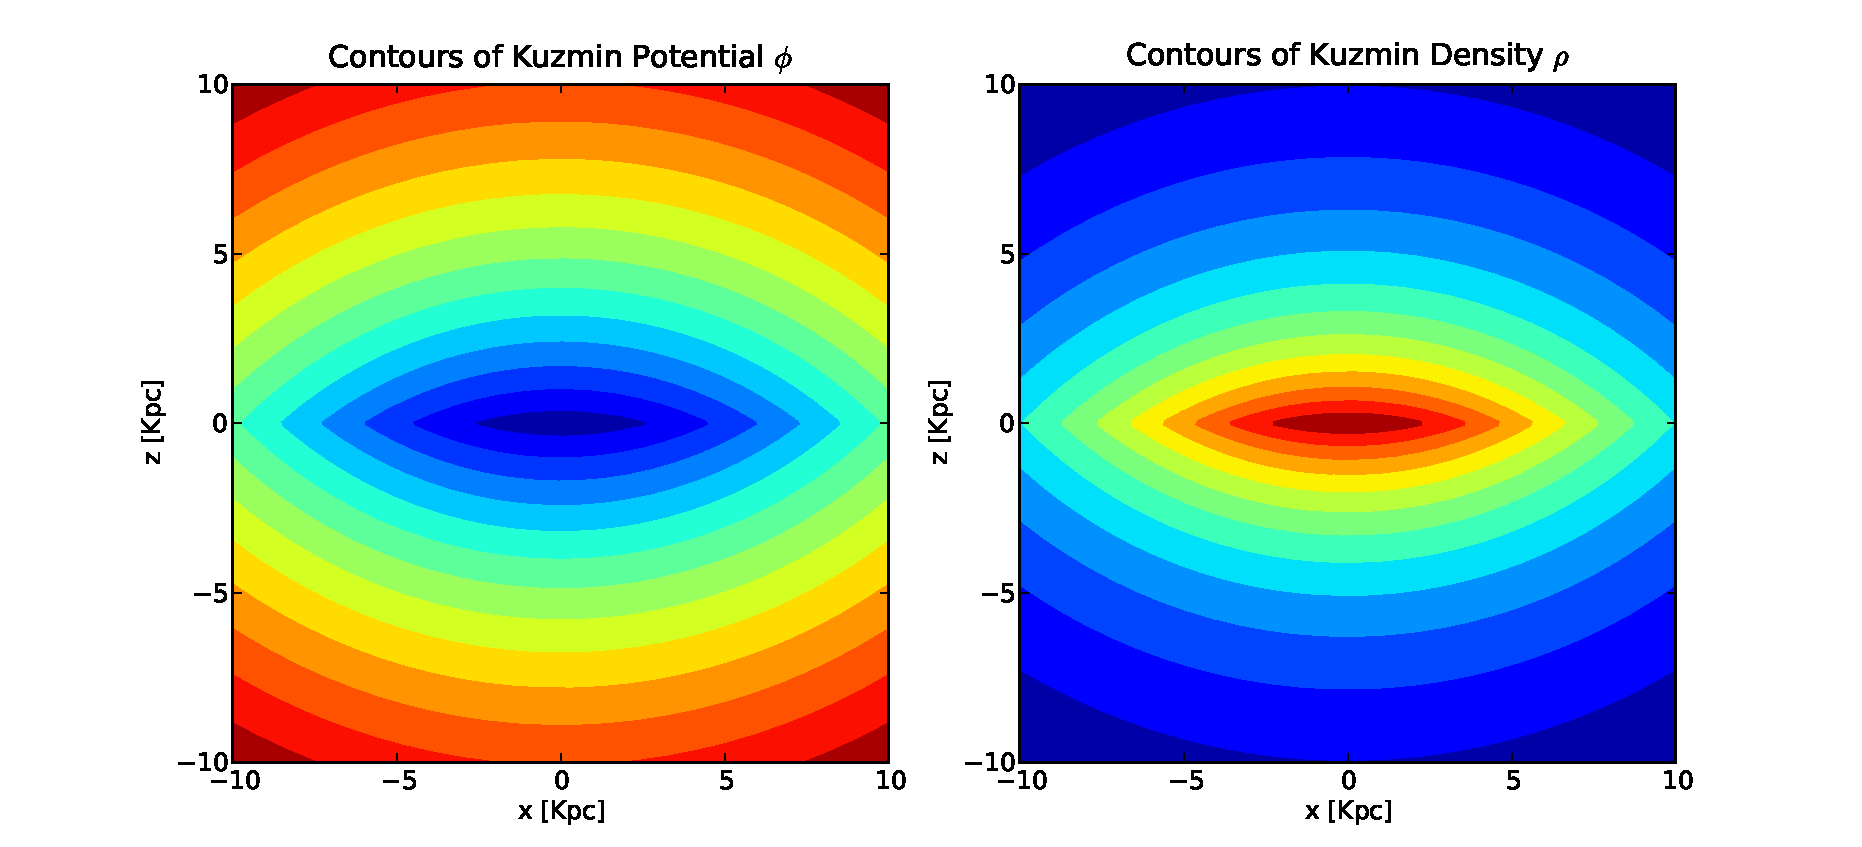
\includegraphics[width=1.0\textwidth]{./figures/figure01.pdf}
	\caption{Par potencial-densidad para un disco logarítmico de Kuzmin.}
	\label{fig:Imagen01}
  \end{figure}
  

\subsubsection*{Disco Logarítmico}
\subsubsection*{Disco Exponencial}

\newpage

%REFERENCIAS ================================================================================

\begin{thebibliography}{}
\bibitem[Kuzmin (1956)]{Kuzmin56}  G.G. Kuzmin, Astron.Zh. 27,33 (1956)

\bibitem[Binney \& Tremaine (1987)]{Binney87} J. Binney \& S. Tremaine: \textit{Galactic Dynamics} (Princenton University Press, Princenton 1987)

\bibitem[Goldstein (1989)]{Goldstein89} H. Goldstein: \textit{Classical Mechanics}, 3th edn (Addison-Wesley, Reading MA, 1989)
\end{thebibliography}

\end{document}